\documentclass[onecolumn, draftclsnofoot,10pt, compsoc]{IEEEtran}

\usepackage{geometry}
\usepackage{natbib}
\usepackage{graphicx}
\usepackage{setspace}
\usepackage{tabularx} % extra features for tabular environment
\usepackage{pgfgantt}
\geometry{textheight=9.5in, textwidth=7in}



% 1. Fill in these details
\def \CapstoneTeamName{		Auction Hunter}
\def \CapstoneTeamNumber{		4}
\def \GroupMemberOne{			Alexander Hull}
\def \GroupMemberTwo{			Alexander Jacobson}
\def \GroupMemberThree{			Yufei Zeng}
\def \CapstoneProjectName{		Auction Hunter}
\def \CapstoneSponsorCompany{	}
\def \CapstoneSponsorPerson{		Ryan Kalb}

% 2. Uncomment the appropriate line below so that the document type works
\def \DocType{		%Problem Statement
				Requirements Document
				%Technology Review
				%Design Document
				%Progress Report
				}
			
\newcommand{\NameSigPair}[1]{\par
\makebox[2.75in][r]{#1} \hfil 	\makebox[3.25in]{\makebox[2.25in]{\hrulefill} \hfill		\makebox[.75in]{\hrulefill}}
\par\vspace{-12pt} \textit{\tiny\noindent
\makebox[2.75in]{} \hfil		\makebox[3.25in]{\makebox[2.25in][r]{Signature} \hfill	\makebox[.75in][r]{Date}}}}
% 3. If the document is not to be signed, uncomment the RENEWcommand below
%\renewcommand{\NameSigPair}[1]{#1}

%%%%%%%%%%%%%%%%%%%%%%%%%%%%%%%%%%%%%%%
\begin{document}
\begin{titlepage}
    \pagenumbering{gobble}
    \begin{singlespace}
    	
\includegraphics[height=4cm]{coe_v_spot1}
        \hfill 
        % 4. If you have a logo, use this includegraphics command to put it on the coversheet.
        %\includegraphics[height=4cm]{CompanyLogo}   
        \par\vspace{.2in}
        \centering
        \scshape{
            \huge CS Capstone \DocType \par
            {\large\today}\par
            \vspace{.5in}
            \textbf{\Huge\CapstoneProjectName}\par
            \vfill
            {\large Prepared for}\par
            \Huge \CapstoneSponsorCompany\par
            \vspace{5pt}
            {\Large\NameSigPair{\CapstoneSponsorPerson}\par}
            {\large Prepared by }\par
            Group\CapstoneTeamNumber\par
            % 5. comment out the line below this one if you do not wish to name your team
            \CapstoneTeamName\par 
            \vspace{5pt}
            {\Large
                \NameSigPair{\GroupMemberOne}\par
                \NameSigPair{\GroupMemberTwo}\par
                \NameSigPair{\GroupMemberThree}\par
            }
            \vspace{20pt}
        }
        \begin{abstract}
        % 6. Fill in your abstract    
        	This document encompasses the features that our proposed product will implement. These features are those requested by our client, and agreed upon by the members of group 4. 
        \end{abstract}     
    \end{singlespace}
\end{titlepage}
\newpage
\pagenumbering{arabic}
\tableofcontents
% 7. uncomment this (if applicable). Consider adding a page break.
%\listoffigures
%\listoftables
\clearpage





\section{Introduction}
\subsection{Purpose}
The purpose of Auction Hunter is to find the highest value car auctions for wrecked/damaged vehicles on auction website.
Our product will parse through a collection of auctions, evaluate their value, and display results to a user through a website UI. 
\subsection{Overview}
There are three primary components to our proposed product. The first part skims over car auctions using a web crawler and collects all relevant data, then saves it. The second part parses through all that saved data and performs estimations on value, which can be compared to the current asking price. The third component displays this information to the user through a website. A user will be able to search for particular characteristics to help narrow down the available auctions. They will also ultimately be the final say over which auction they choose. Images of each auction will be displayed to the user, which enables them to make a final judgment call. A stretch goal would be to use machine learning to eliminate or promote a subset of auctions based on the images provided.

\subsection{Definitions}
Web Crawler - a program that systematically collects information off of the web. This can be used to compile information or data without requiring a human to manually navigate to each web page. 

Website UI - A privately or publicly hosted website which will use an internet browser to display information to a user. It serves as a way for humans to easily interpret information that is being collected and calculated upon in the back-end. 

Wrecked Car Auctions - Insurance companies will commonly create auctions to sell cars that have crashed or been badly damaged. The insurance company will pay out an insurance holder, or replace their car. Vehicles are commonly auctioned because insurance companies avoid repairing them due to high or variable repair costs. 

Highest Value Car - The cars being sold at auction have some intrinsic value. This could be the grand total of each individual part after labor has been accounted for. It could also be the total price of the car after necessary repairs have been performed. Since the cars are sold at auction, this price is more variable based on bidders' actions. An auction would be worth bidding on if the total value is greater than the current asking price. Since there are so many auctions, the best would be displayed first. 

\section{System Requirements}
A publicly hosted Auction Hunter website that displays to the user the projected value of each auction. There will also be a way for the user to sort the list of auctions to refine their search. When a user finds a high value action, they can obtain additional information such as images and a link to the original auction listing. 

This website will utilize a number of back-end scripts which crawl through wrecked car auctions to pull all relevant data. Once the data from each auction is collected, we can predict relative values for each auction and add it to a database to be displayed to the user. 

To better judge the effectiveness of our algorithms, we can compare the value that our scripts assign to each car to the final sale price. We can also manually evaluate our predictive algorithms to verify it is assigning value correctly. We will plot any relevant performance data to present the effectiveness of our algorithms.  

%\section{System Requirements}

\subsection{User Stories}
\begin{itemize}
\item As a user, I want to be able to access Auction Hunter from anywhere.
\item As a user, I want a user interface that is easy to use.
\item As a user, I want to sort the car list by selecting price range and present or absence of VIN. 
\item To save as much money as possible, I want to make sure that I am getting a good deal on wrecked car auctions, especially for newer vehicles.
\item As a user, I want to be able to set alerts when there is a car I want up for auction
\item As a mechanic, I want to have proof that Auction Hunter is accurate in it's value predictions so I can buy parts while saving money. I also want proof that it works faster than manually evaluating auctions.
\item Auction Hunter should be able to scrape Auction data from IAAI and be extendable to scrape other sources.
\end{itemize}

\subsection{Functional Requirements}
At its core Auction Hunter is a website that allows users access to information it has stored in its database. The website should allow for the following functions to be preformed.

\begin{itemize}
\item User access controls to only allow signed-up users access to the Auction Hunter
\begin{itemize}
    \item Allow users to sign up to Auction Hunter
    \item Let users sign in using their email and password
    \item Reset their password if a user forgets it
\end{itemize}
\item Account page to manage user preferences
\begin{itemize}
    \item Lets user change email and password
    \item View notifications Auction Hunter has sent them about auctions
    \item Specify parameters about what types of auctions they want alerts about
\end{itemize}
\item Details page that display all information about a specific auction
\begin{itemize}
    \item Pictures of car
    \item Estimated value of car calculated by Auction Hunter
    \item All other data that Auction Hunter can find on auction websites
\end{itemize}
\end{itemize}

Auction Hunter also needs a way of gathering the auction data to power its website. This is done via web scraping scripts that run at automated times.

\begin{itemize}
    \item Scrape IAAI website for basic auction data
    \begin{itemize}
        \item Vin
        \item Damage information
        \item Start Code
        \item Presence of key
        \item Link to original posting
        \item Airbag and crash data
        \item Photos of vehicle and damage
        \item Options and specifics of the car
    \end{itemize}
    \item Scrape auction websites for when auctions are happening in the future
\end{itemize}

\subsection{Performance requirements}
Response Time: All of the response time are measured in end user environment(the browser rendering the response)
\begin{itemize}
\item Below operations must respond within 5 seconds.
\begin{itemize}
    \item “Access action hunter homepage”
    \item “Sign up”
    \item “Log in account”
    \item “Log out account”
    \item "Viewing the details of car"
    \item “Set the values of notification for coming cars”  
    \item “Sort the list of auctions by price, value, model, VIN, etc”
\end{itemize}
\end{itemize}

\begin{center}
Workload: The table below estimates that for a user scenario how many requests per day.\\
\begin{tabular}{ | m{2cm} | m{4cm}| m{3cm} | m{3cm} | } 
\hline
Ref No & Scenario & Pages & Daily Total(estimate) \\ \hline
1 &Visit homepage   &Portal  &100\\  
\hline
2 &Sort car list  &Portal  &100\\
\hline
3 &Set notification  &Login,Notification  &10\\
\hline
\hline
4 &Scrape auction data  &Portal  &80\\
\hline
5 &View notification  &Login,Notification  &10\\
\hline
6 &View bid  &Login,Bid  &5\\
\hline
7 &View car details  &Portal,CarDetails &90\\
\hline
\end{tabular}
\end{center}


\subsection{User Testing}
As a stretch goal, we could get some users unaffiliated with this project to try out our final website to provide feedback. 


\section{Schedule}
\begin{ganttchart}[hgrid,vgrid]{1}{28}
    %Fall
    \gantttitle{2018-2019 By Week (Ignoring Breaks)}{28} \\
    \gantttitlelist{1,...,28}{1} \\
    \ganttgroup{Fall 2018}{1}{6} \\
    \ganttgroup{Winter 2019}{7}{17} \\
    \ganttgroup{Spring 2019}{18}{28} \\
    \ganttbar{Requirements Draft}{1}{2} \\
    \ganttlinkedbar{Requirements Final}{3}{5} \\
    \ganttbar{Tech Review Draft}{1}{2} \\
    \ganttbar{Design Document}{4}{6} \\
    \ganttlinkedbar{Client Verification}{5}{6} \\
    \ganttbar{Info Interview}{5}{6} \\
    
    %Winter
    \ganttbar{Basic Web Crawling}{7}{9}\\
    \ganttlinkedbar{Backend Database}{8}{10}\\
    \ganttlinkedbar{Website }{10}{13}\\
    \ganttlinkedbar{Value Calc}{8}{12}\\
    \ganttlinkedbar{Incorporate Components}{13}{17}\\
    
    
    %Spring
    \ganttbar{Finalize Implementation}{18}{20}\\
    \ganttlinkedbar{Verification}{20}{22}\\
    \ganttlinkedbar{Real world testing}{22}{24}\\
    \ganttlinkedbar{Prepare for expo}{24}{28}\\
    
    %\ganttlinkedbar{Task 2}{3}{7} \ganttnewline
    \ganttmilestone{Expo}{28} \ganttnewline
\end{ganttchart}

\begin{figure}[ht]
\centering
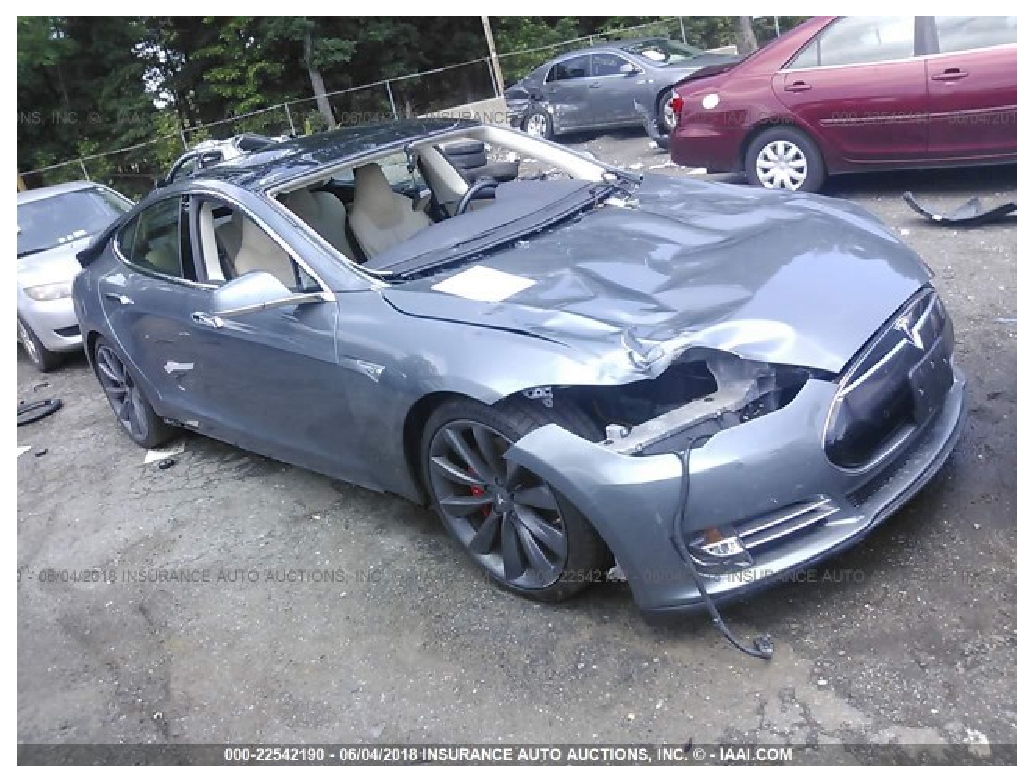
\includegraphics{model-s.eps}
\caption{Example of salvage car to be auctioned}
\label{fig:flow}
\end{figure}



\end{document}
